\subsection{Schiefwinklige Dreiecke}
\label{subsec:fundamentals_oblique_triangles}

Neben rechtwinkligen Dreiecken treten Dreiecke ohne rechten Winkel auf. Für
sie liefern Sinus- und Kosinussatz die benötigten Beziehungen zwischen Seiten
und Winkeln.

\begin{DefinitionBox}{Schiefwinkliges Dreieck}{fundamentals_oblique_triangle}
  Ein \emph{schiefwinkliges Dreieck} \EnglishTerm{oblique triangle} ist ein
  Dreieck, das keinen rechten Winkel besitzt.

  \begin{center}
    \CachedTikzFigure{content/resources/chapters/fundamentals/tikz/oblique_triangle.tex}
  \end{center}
\end{DefinitionBox}

\begin{RemarkBox}
  Ohne rechten Winkel gibt es keine Hypotenuse und keine Katheten. Die Seiten
  werden ausschließlich über die jeweils gegenüberliegenden Winkel
  zugeordnet.
\end{RemarkBox}

\subsubsection{Sinussatz}
\label{subsubsec:fundamentals_oblique_triangles_sine_rule}

Die Höhe $h$ zerlegt das schiefwinklige Dreieck in zwei rechtwinklige
Dreiecke. Dadurch lässt sich der Sinussatz aus den bereits bekannten
Seitenverhältnissen herleiten.

\begin{center}
  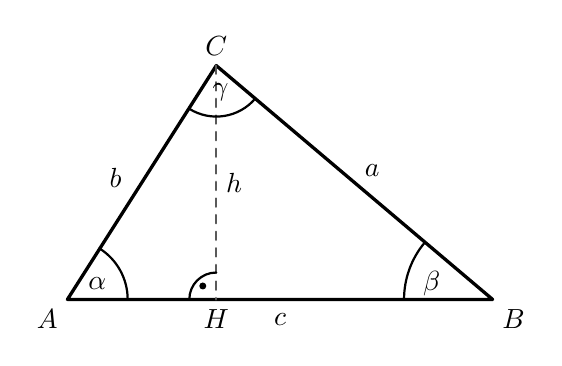
\begin{tikzpicture}[scale=0.9,line cap=round,line join=round]
  \coordinate (A) at (0,0);
  \coordinate (B) at (6,0);
  \coordinate (C) at (2.1,3.3);
  \coordinate (H) at (2.1,0);

  \draw[very thick] (A) -- (B) -- (C) -- cycle;
  \draw[thick,dashed,black!65] (C) -- (H);

  \node[below left] at (A) {$A$};
  \node[below right] at (B) {$B$};
  \node[above] at (C) {$C$};
  \node[below] at (H) {$H$};

  \node at (4.30,1.82) {$a$};
  \node at (0.68,1.72) {$b$};
  \node at (3,-0.28) {$c$};
  \node[right] at (2.1,1.65) {$h$};

  \draw[thick] (0.85,0) arc[start angle=0,end angle=58,radius=0.85];
  \node at (0.42,0.23) {$\alpha$};
  \draw[thick] (4.75,0) arc[start angle=180,end angle=140,radius=1.25];
  \node at (5.14,0.23) {$\beta$};

  \draw[thick] (1.72,2.69) arc[start angle=-122,end angle=-40,radius=0.72];
  \node at (2.16,2.93) {$\gamma$};

  \draw[thick] (2.1,0.38) arc[start angle=90,end angle=180,radius=0.38];
  \fill (1.91,0.19) circle (1.4pt);
\end{tikzpicture}

\end{center}

In den beiden rechtwinkligen Teildreiecken gilt
\begin{ClozeArea}[34]{9}
  \[
    \left.
    \begin{aligned}
      \text{linkes Dreieck:}\quad &\sin(\alpha)=\frac{h}{b},\\
      \text{rechtes Dreieck:}\quad &\sin(\beta)=\frac{h}{a}
    \end{aligned}
    \right\}
    \quad\Longrightarrow\quad
    b\sin(\alpha)=h=a\sin(\beta).
  \]
\end{ClozeArea}

\begin{TheoremBox}{Sinussatz}{fundamentals_sine_rule}
  In jedem Dreieck verhalten sich die Seitenlängen wie die Sinuswerte der
  jeweils gegenüberliegenden Winkel:
  \begin{ClozeArea}[27]{5}
    \[
      \frac{a}{\sin(\alpha)}
      =\frac{b}{\sin(\beta)}
      =\frac{c}{\sin(\gamma)}.
    \]
  \end{ClozeArea}
\end{TheoremBox}

\subsubsection{Kosinussatz}
\label{subsubsec:fundamentals_oblique_triangles_cosine_rule}

Der Kosinussatz verallgemeinert den Satz des Pythagoras auf beliebige
Dreiecke. Neben drei Seitenlängen tritt dabei der eingeschlossene Winkel auf.

\begin{TheoremBox}{Kosinussatz}{fundamentals_cosine_rule}
  In einem beliebigen Dreieck gilt
  \begin{ClozeArea}[27]{5}
    \[
      c^2=a^2+b^2-2ab\cos(\gamma).
    \]
  \end{ClozeArea}
  Dabei liegt der Winkel $\gamma$ der Seite $c$ gegenüber.
\end{TheoremBox}

Da keine Seite ausgezeichnet ist, kann dieselbe Beziehung für jede Seite
formuliert werden:
\begin{ClozeArea}[30]{8}
  \begin{align*}
    a^2&=b^2+c^2-2bc\cos(\alpha),\\
    b^2&=a^2+c^2-2ac\cos(\beta),\\
    c^2&=a^2+b^2-2ab\cos(\gamma).
  \end{align*}
\end{ClozeArea}

\begin{RemarkBox}
  Für $\gamma=90^\circ$ ist $\cos(\gamma)=0$. Damit geht der Kosinussatz in
  den Satz des Pythagoras über:
  \[
    c^2=a^2+b^2-2ab\underbrace{\cos(90^\circ)}_{=0}=a^2+b^2.
  \]
\end{RemarkBox}

